% Project Specifications
\clearpage%if the chapter heading starts close to bottom of the page, force a line break and remove the vertical vspace
\vspace{21.5pt}
\chapter{Project Specifications/Background}

To perform the needed recovery operations as described in the previous section the project has to be able to perform several operations. Both standard Raspberry Pi Pico and Raspberry Pi Pico W are going to be used, so the project should be able to support both board types and automatically detect the correct attached target type without user interaction.

Software images for both board types thus have to be stored on the recovery board, and a method to update the stores images. Preferably this image updating would be handled fully by the recovery board itself, without using some form of accompanying image rebuilder on a computer, in order to keep platform independence and simplicity of operation.

The project should be able to interface with a target board to query file system status and perform file system operations to recover target board from potential non booting status, including zeroing out full file system to perform a quick reset, or reimage a full firmware to target board.

This project is specified to be done using a Raspberry Pi Pico operating standalone without a computer for convenience to use existing resources, and as a potential demonstration of a use for a Pi Pico.

\clearpage
\section{Hardware}

\subsection{Overview of Raspberry Pi Pico}

\begin{figure}[ht]
	\centering
	\AltText{Stock photo of Raspberry Pi Pico}{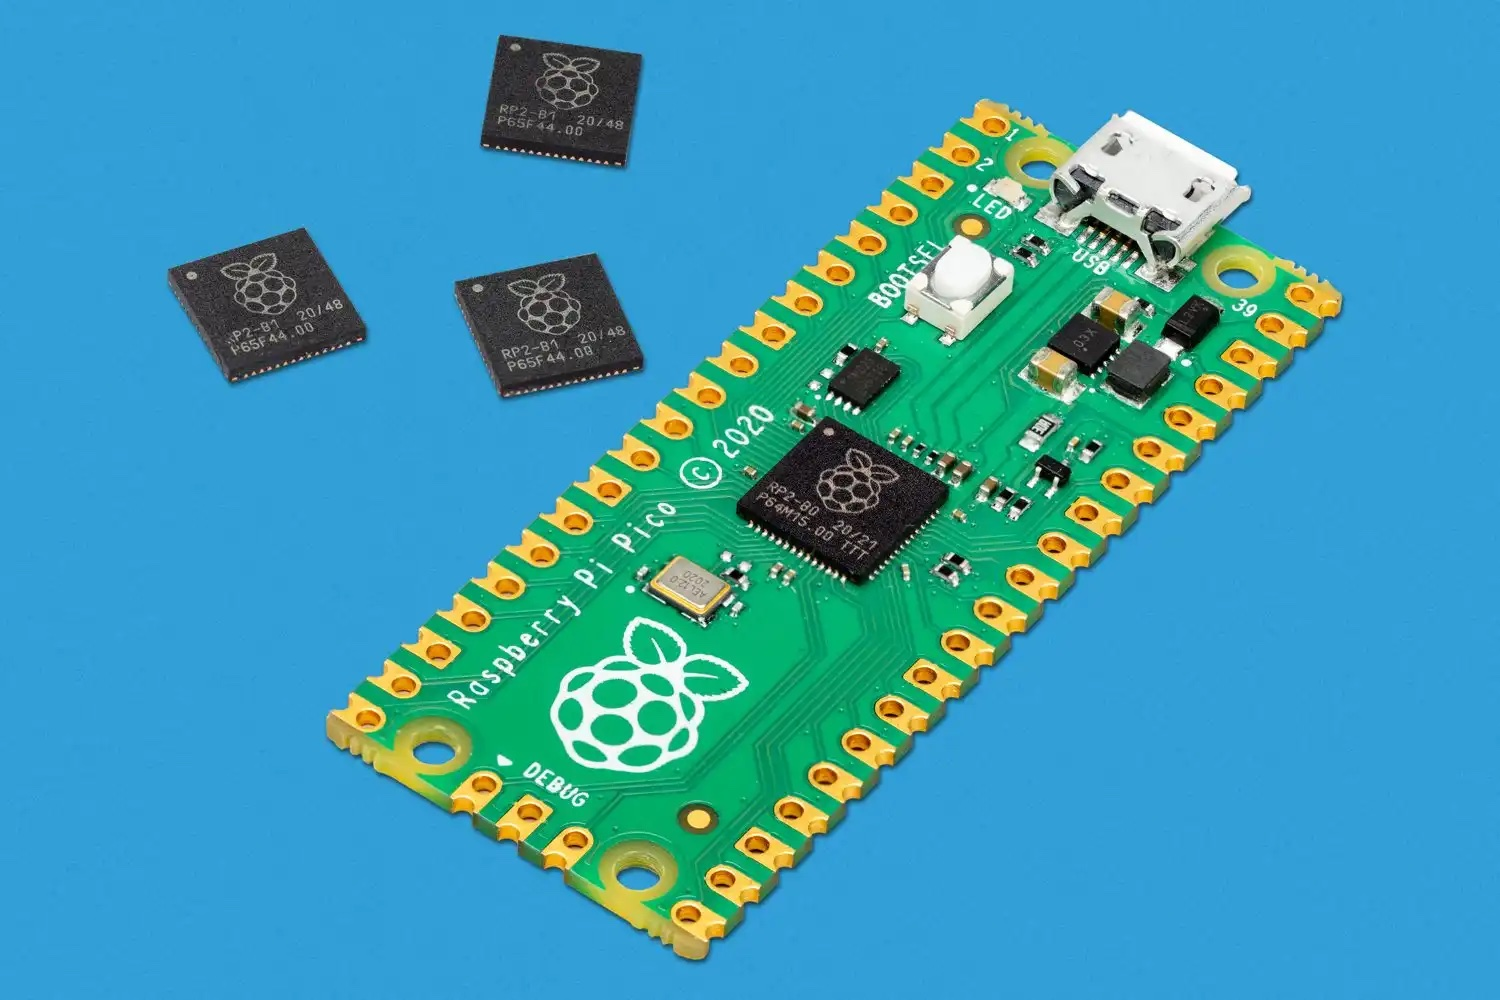
\includegraphics[width=\textwidth]{pico-rp2040}}
	\caption{Stock photo of Raspberry Pi Pico\cite{ltdBuyRaspberryPi}}
	\label{fig:picostock}
\end{figure}

The principle target recovery baord and project board are both a Raspberry Pi Pico \autoref{fig:picostock} which is a compact \gls{mcu} development platform created by the Raspberry Pi Foundation, running a dual core \gls{arm} Cortex M0 at 133Mhz with a larger than typical 264kB inbuilt \gls{ram} and 2MB of \gls{spi} flash memory storage for the class of \gls{mcu}\cite{ltdBuyRaspberryPi}.

The Pi Pico is relatively unusual for a \gls{mcu} in not containing any internal program execution flash memory, with programs executing either directly from RAM with boot time wait and upload, or more commonly directly out of attached \gls{qspi} flash with \gls{xip} functionality. External flash access is inherently much slower than normal internal programmable ROM flash due to the \gls{spi} bus, but to aid in achieving near equivalent execution speed the Pico has a configurable \gls{xip} hardware module that by default utilises 16kB of it's internal RAM as a cache for code execution, which is automatically maintained by the hardware. This \gls{xip} design is one of the ways the price of the Pi Pico is kept low, as only one silicon package design is needed unlike typical \gls{mcu}'s that come in a variety of configurations with different flash package sizes depending upon need, whilst also allowing much larger storage sizes without complicating software design as the full external \gls{spi} flash is mapped directly into address space by the inbuilt ROM library.

%TODO: Why not talk about pico XIP? Executing code directly out of SPI flash is quite unique concept  DONE

%The Pico is capable of having it's software image programmed to it via inbuilt ROM USB flasher using a UF2 image or via \gls{swd} interface.

\clearpage
\subsection{Pico Display Pack}
A Pimoroni Pico DIsplay Pack\autoref{fig:picodisplaypack} was selected as the user interface hardware for development due to availability on hand, but is a non critical component that could be swapped for other displays and input with relatively minor adjustment.

The Display Pack features four tactile buttons and a 1.14” 240x135 pixel IPS LCD screen to allow user feedback and input in order to allow a feedback interface for following progress in a more user friendly manner than something akin to a set of simple status LED's which would be hard to intuitively interpret.

\begin{figure}[ht]
	\centering
	\AltText{Stock photo of Pimoroni Pico DIsplay Pack}{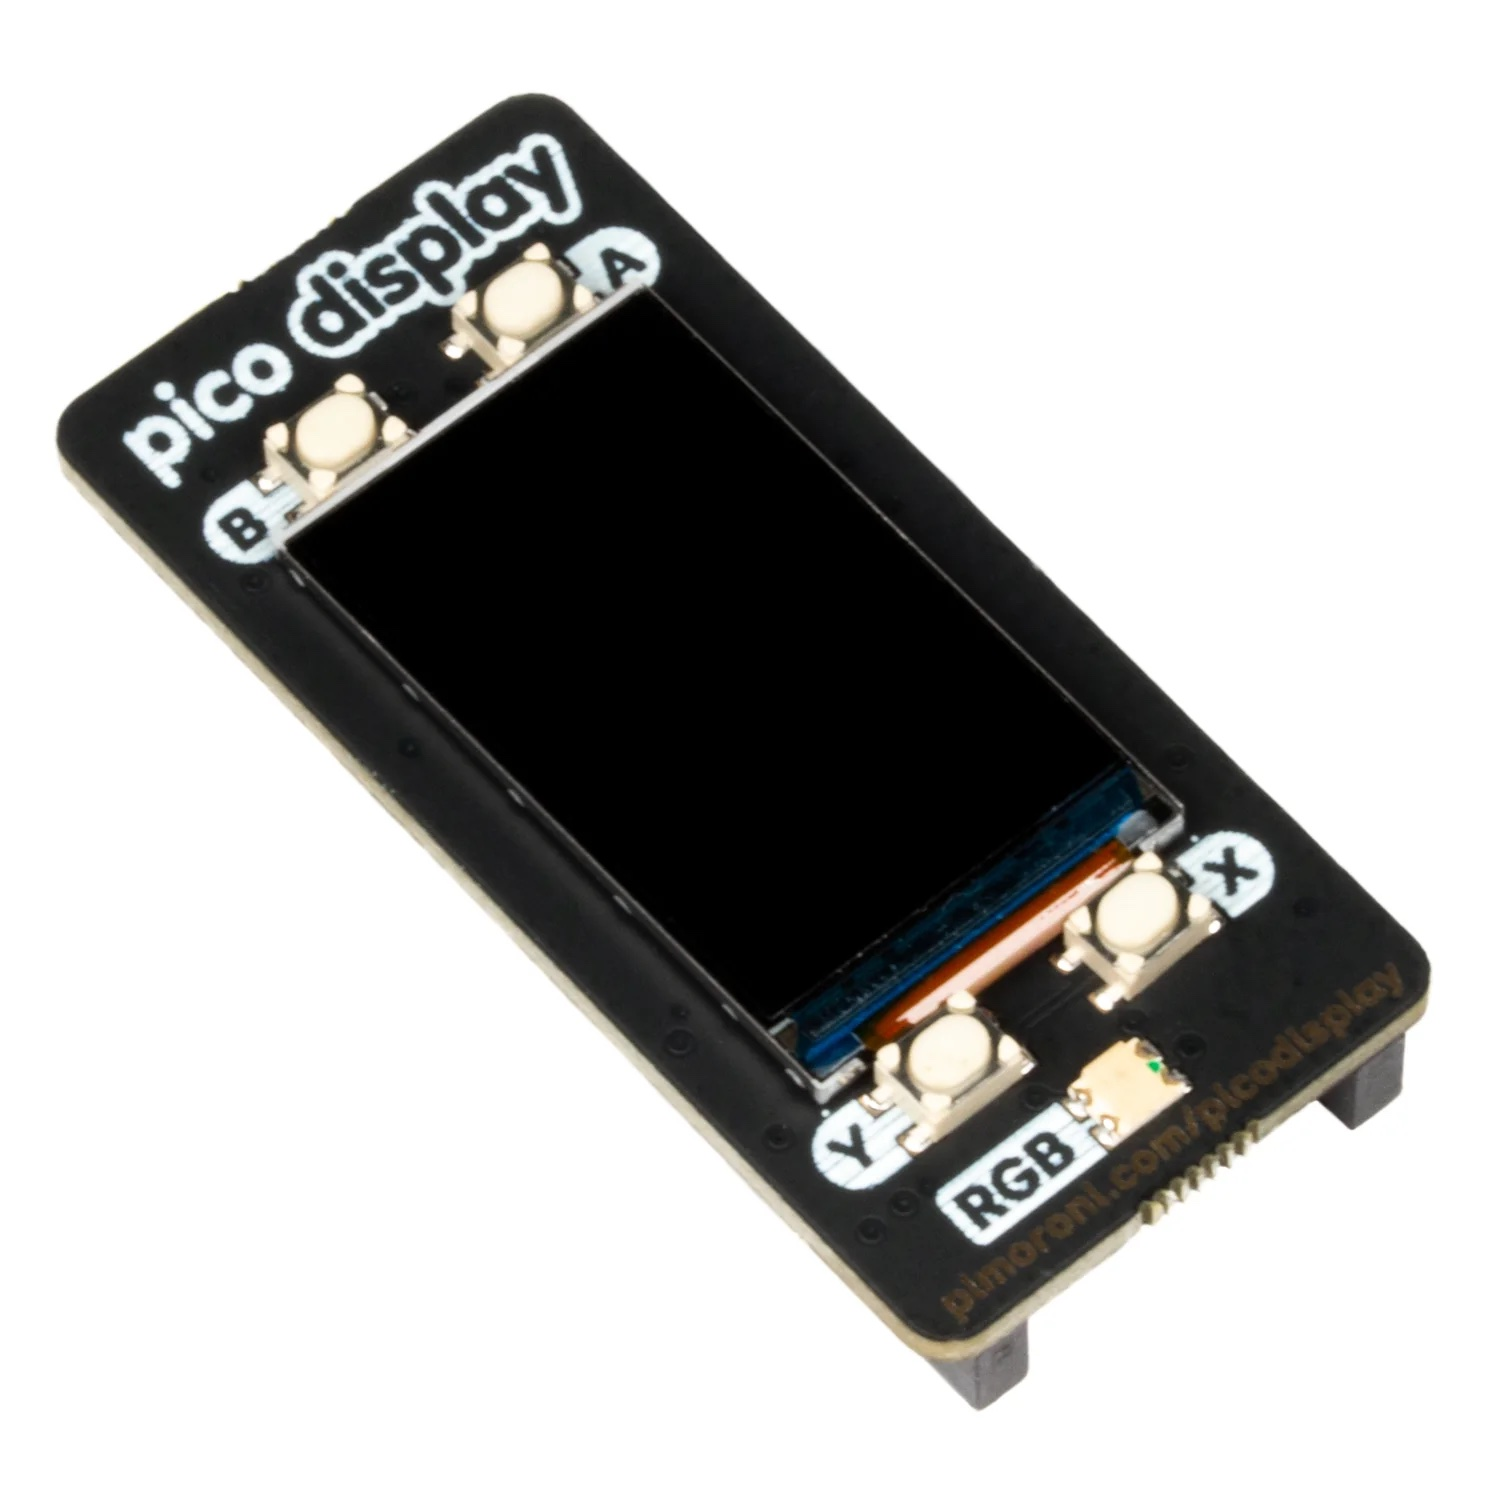
\includegraphics[width=.66\textwidth]{picodisplaypack}}
	\caption{Stock photo of Pimoroni Pico DIsplay Pack\cite{PicoDisplayPack}}
	\label{fig:picodisplaypack}
\end{figure}
	
\clearpage
\subsection{J-Link EDU Mini}
For debugging and rapid prototyping a J-Link EDU Mini\cite{JLinkEDUMini}\autoref{fig:jlinkedumini} from SEGGER GmbH was used as the hardware debugger for project to enable rapid development and debugging without constant manual image upload cycles during testing.

This is a \gls{usb} compact hardware debugger for embedded platforms to provide direct flashing and debug access to the Pi Pico to provide a more convenient development environment with one click compiling and target flashing, and allows utilisation of SEGGER's RTT library for debug messaging output and debug testing commands with low impact to operational performance and no extraneous hardware interfaces.

\begin{figure}[ht]
	\centering
	\AltText{Stock photo of J-Link EDU Mini}{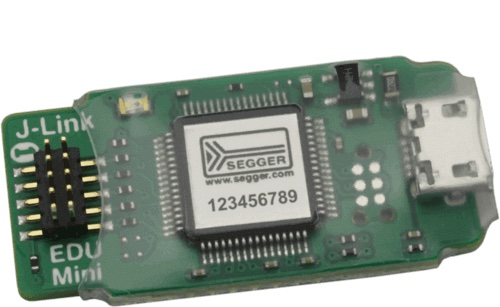
\includegraphics[width=.66\textwidth]{jlinkedumini}}
	\caption{Stock photo of J-Link EDU mini\cite{JLinkEDUMini}}
	\label{fig:jlinkedumini}
\end{figure}

\clearpage
\section{Ways to access Raspberry Pi Pico flash}

There are a couple of potential ways to be able to access the flash memory on the pico to be able to alter or reflash it as desired, with the most common and usually used method for uploading software images performed by holding down the 'BOOTSEL' button when plugging the Pi into \gls{usb}, which disabled the \gls{qspi} flash memory chip select line temporarily during boot process and causes the \gls{mcu} to automatically go into flashing mode whereupon the chip presents a virtual fat drive as a mass storage device to the \gls{usb} host allowing an image to be dragged on and flashed.

Whilst there is a standard \gls{spi} protocol for accessing flash modules, this is limited to 24 bit addressing over a single \gls{spi} lane which limits default \gls{rom} access to a maximum of 16 Megabytes at slow speeds. In order to allow larger module sizes and faster operation speeds \gls{qspi} is supported, which allows 4 bit parallel data transfer for fast operation, but due to lack of standardisation for initialising and accessing these modules in full address space and speed custom initialisation code is needed per device.

In order to allow the inbuilt hardcoded Pi Pico \gls{rom} bootloader to be able to run code directly via \gls{xip} on any possible \gls{spi} module, current or future without limitations, a small secondary bootloader called boot2 is required to be placed at the start of the flash module which is loaded by the \gls{rom} bootloader using standard SPI protocols. This boot2 image is responsible for initialising the specific module to which software image has been targetted and starting final program execution, and is normally managed by the Pico SDK project setup where flash type is specified.

%TODO You should also describe the normal bootloading process and what options you have there. There is a secondary bootloader (or config) on the flash... Done

This method could be used to run a \gls{ram} resident program via specific UF2 loading addresses which could be used to examine the flash memory and run an automatic recovery of a filesystem from MicroPython without affecting the primary flashed application.

But this method is cumbersome, as it cannot be fully automated due to the requirement of manual BOOTSEL enablement to enable whilst plugging in. There are ways to enter recovery mode without pressing BOOTSEL via \gls{usb} interface using picotool application that can make negotiate a pico running firmwares based on standard \gls{usb} stack to reboot into recovery mode\cite{picotool}, but this is inflexible and would not help recovering an application that immediately disables USB automatically at boot which is one of the primary requirements of the project.

The other principle method of being able to arbitrarily access flash memory on pico is via the \gls{arm} \gls{swd} debug interface using the board accessible debug pads intended for direct programming and onchip debugging\cite{ARMDebugInterface}.

The \gls{swd} interface  is always available regardless of firmware setup, and allows full control of the chip thus making it possible to fully automate. The principle disadvantage of this approach is the less convenient physical access to the interface compared to connecting to a \gls{usb} host.
\clearpage
\section{SWD interface}
The \gls{arm} \gls{swd} interface is an \gls{arm} microdevices created standard for all \gls{arm} Cortex CPU's using two wires for clock and signal, that allows bidirectional communication over a single signal wire and a variable host controlled signal speed.

Typical \gls{swd} control speeds range from 4-25MHZ clock, though to achieve high clock rates typically seperate hardware such an \gls{fpga} programmed for dedicated signal control is used. Bue due to the debugger controlled clock, timing is not critical and can be flexible allowing a more simplistic 'bit banging' approach to be used from any GPIO interface, though more refined methods utilising peripheral hardware inside an \gls{mcu} can be possible, such as \gls{spi} controller, or in the case of the Pi Pico there is a relatively unique {\gls{pio} hardware interface that can be utilised for \gls{swd} as utilised in the Raspberry Pi Foundations Pi Pico based debug probe.

\gls{pio} is in effect a pair of smaller very simple tertiary sub processor modules on the pico that run state machines dedicated to \gls{gpio} processing using a custom Assembly language that allow custom protocols to be implemented in a flexible way with tight hardware timing without the inconvenience of processor interrupts which make achieving such processing with a tightly controlled timing almost impossible with software controlled \gls{gpio} outside all but the simplest control systems.

%TODO  Maybe a few words about pio assembly here? DONE

Communication with the debug unit is first established with a reset sequence, which will always reset the debug unit to a known starting state so that connection can be established regardless of existing state.

Every transaction consists of a multiple phase process. First a request header to signal read or write a register including contained command validation parity check is clocked out onto the \gls{swd} I/O line, after which the host switches to reading the I/O line and clocks in three bits to check for an acknowledgement reply indicating whether the request was received, debug unit is busy or can action the request, or if the debug unit is in fault state.

If the acknowledgement is an all OK, then the next action is either clocking in the bus for length of data to read response, or switching back to clocking out the transmitted data packet. In the case of \gls{ap} memory reads, the first data read after a initial read request has to be ignored and discarded to give the debug unit time to retrieve the memory data, thus read cycle will always have an extra throwaway read at the end also.

After a data transfer if no other command is to be immediately processed an extra 8 clock cycle idle has to be continued post transfer to allow the debug unit to process requests internally such as memory writes. This ensures that the debugger is not left in an unknown state of execution which could result in unexpected behaviour.

\begin{figure}[ht]
	\centering
	\AltText{Diagram of ARM SWD memory write operation}{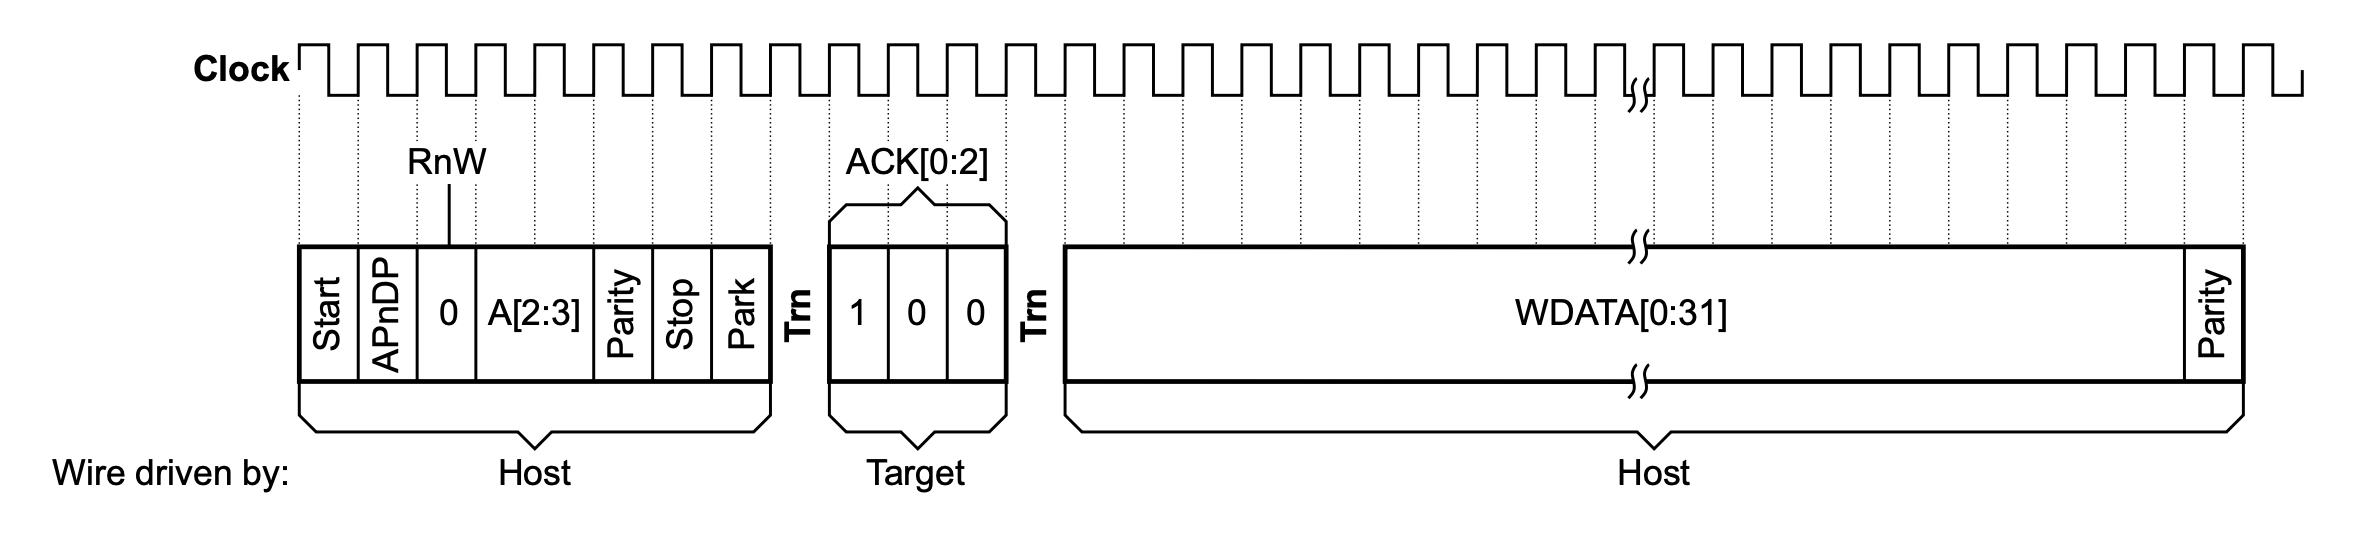
\includegraphics[width=\textwidth]{armswdwrite}}
	\caption{Diagram of SWD memory write\cite{ARMDebugInterface}}
	\label{fig:armswdwrite}
\end{figure}

\gls{arm} \gls{mcu}'s can also optionally support \gls{jtag} protocol debugging, using the same pins as \gls{swd}. For chips supporting both a handshake to establish the protocol being used is needed. But as the Pico is an \gls{swd} only \gls{mcu}, this part of the connection protocol is not needed which simplifies initialisation for the target device.

Each CPU core has it's own debug unit, along with a third 'reset' unit that can be used to reset the whole \gls{mcu}, and \gls{swd} control allows commanding the debug units in the \gls{mcu}, which allows reading and writeing memory, control of execution including setting breakpoints and other debug aiding measures.

\gls{swd} cannot directly access the flash memory on the Pico as this is external to the \gls{cpu}, and in order to perform operations on flash memory via debug interface the \gls{mcu} has to be instructed in some manner using memory access and process control to perform the operations required indirectly. This can be done via direct instructions to perform required actions which are first written into memory whilst core is halted or waiting before a jump and execute is instructed step by step for direct flash programming, though this would be very inefficient due to amount of waiting for writes and instructions to be prepared and waited for. A simpler and more reliable method which is typically used for flash programming via debuggers is uploading a small stub flash loader application with which the debugger communicates via a defined shared memory space, where some form of flashing cache buffer can be filled for the stub to continue programming.

For controlling the \gls{swd} interface there are two main possible methods to consider. Firstly so called 'bit banging' \gls{gpio} signals utilising \gls{arm} code to control signal lines via direct access which is effectively entirely non hardware dependant. Secondly using a \gls{pio} module in the Pico which would allow a lower level clock accurate control of \gls{gpio} on the device, an example implementation of which available in the official Raspberry Pi Pico debugger PicoProbe project\cite{Picoprobe2023}. It is also potentially possible to utilise \gls{spi} peripheral in order to perform \gls{swd} transactions, though this was deemed unnecessarily complicated to investigate as a potential solution compared to the main methods already discussed.\cite{OpenOCDRaspberryPi}.

Due to \gls{swd}'s use of host device clock signal and no tight timing requirements for it's operation, the simpler software based 'bit banging' was implemented as first proof of concept, which combined with running the pico clock at a technically overclocked but still stable 230 Mhz operating speed allowed faster timing in a simple manner opposed to implementing a more complex pio based solution.

%TODO:  SW based or pio assembly?  DONE

\clearpage
\section{Helper Binary Image}
In order to perform operations on the target device in an efficient manner without directly writing instructions to target memory for every operation a secondary memory resident helper application image is needed, which is embedded within the recovery flasher's image and uploaded to the target device on initialisation. The helper application is responsible for performing the actual recovery processes on the target hardware, such as reporting target hardware type to the recovery board using a detection routine based on ADC3 readings from voltage regulator depending upon a \gls{gpio} pin state that differs between Pico and Pico Wireless\cite{IdentifyingPicoPicoW}, reading /writing flash image and performing file system accesses and modifications.

Flash access is done in the helper application by calling into inbuilt bootloader ROM library routines on the target Pico to perform inbuilt default \gls{spi} flash initialisation to map external flash into address space and enable default ROM flash write routines to be callable for write operations in the same compatible manner the inbuilt BOOTSEL flasher performs. Due to the access speed requirements of flashing being lower than execution and necessary software image file system being within the default 24 bit address area of standard \gls{spi} flash access, no further boot2 initialisation for full flash chip capability is needed, mirroring normal BOOTSEL flash image write process.

\clearpage
\section{USB Flashing Format}
\gls{uf2} is a file format created by Microsoft with the intention of having a simple universal file format for device firmware image updates, that is very easy to support with a minimal loader to manage the flashing on target device, intended primarily for use via a \gls{usb} supporting bootloader that presents a virtual file system to the operating system via standard \gls{usb} \gls{msc} protocol, so that special hardware and software is not needed for firmware updates.

A \gls{uf2} file is composed of a series of 512 byte blocks, each of which consists of an identifying header, payload, and a closing end magic number to verify receipt of complete blocks\autoref{table:uf2header}. The Payload can be upto 476 bytes, but typically only 256 bytes are actually used to in order to align with flash block write sizes, helping keep block addressing simple. This typical underutilisation of payload allocation leads to a notable percentage of wasted space within files but ensures that file system writes over virtual \gls{usb} \gls{msc} always contain complete blocks\cite{USBFlashingFormat2023} allowing capturing and writing data to flash without buffering multiple writes in normal usage which simplifies flasher design. 

The 32 byte header of each block contains necessary information to direct flashing process such as the payloads destination flash address in \gls{rom}, a family code to verify device type the image is meant for, the relative number of current block, and a total block count for complete image.

\gls{uf2} block header also contains a flag field which allow s further optional features in the format, including a checksum for the data and presence of family type instead of file size which is typically used instead of the default file size field, as family field is useful to help prevent incorrect firmware uploads to desce and complete firmware image size being calculable from the stored block count data and assumption of typical payload size. Checksum data is not typically used, and thus not needed to be implemented.

This is enough information for flashing software to know where to put each part of image as received, and keep track of progress in order to know full image has been received without an explicit end of transfer or blocks received out of order, which is key to being able to flash images via \gls{usb} \gls{msc} file system write.

The format was chosen by the Pi foundation as the native image format for the pico due to this simplicity of use, and the pico recovery bootloader presents a \gls{usb} mass storage virtual \gls{fat} file system from it's \gls{rom} stored 16kB alongside \gls{usb} stack and \gls{rom} callable routines for functionality including \gls{spi} flashrom writing. When reading in an image the bootloader uses the target address of the image to signify whether to load the data into ram for immediate execution, or to flash and execute from \gls{qspi}.

\begin{table}[h]
	\centering
	\caption{UF2 Format Block header\cite{USBFlashingFormat2023}}%IMPORTANT the caption must be before the tabular, so it will be on top of the table (there are other tricks to force it on top; but this one is straightforward).
	\vspace{-16.5pt}%time to time, spacing between caption and table can go too big...
	
	\begin{tabular}{|l|l|l|}
		\hline
		Offset	& Size &	Value\\ \hline
		0	& 4 &	First magic number, 0x0A324655 ("UF2\textbackslash n")\\ \hline
		4&	4&	Second magic number, 0x9E5D5157\\ \hline
		8	&4&	Flags\\ \hline
		12&	4	&Address in flash where the data should be written\\ \hline
		16&	4	&Number of bytes used in data (often 256)\\ \hline
		20&	4	&Sequential block number; starts at 0\\ \hline
		24&	4	&Total number of blocks in file\\ \hline
		28&	4	&File size or board family ID or zero\\ \hline
		32&	476&	Data, padded with zeros\\ \hline
		508&	4&	Final magic number, 0x0AB16F30\\ \hline

	\end{tabular}
	\label{table:uf2header}
\end{table}

\clearpage
\section{USB Virtual Filesystem}
Standalone \gls{swd} control is enough to be able to recover a file system or erase a board to rescue bootloader state, but in order to fully setup a Pico from scratch a flash image to program is needed. This image could be included into the program as a binary include, but this makes updating cumbersome requiring recompiling and uploading a new full binary image to the recovery Pico, which is typically achieved by setting the Pico into BOOTSEL recovery mode and flashing the new combined \gls{uf2} image on.

It was figured that a more convenient alternative would be for the device to manage it's own images, which also allows device to signal what firmware is installed to the user via filename, and due to the requirement to support both Pico original and wireless editions, two separate firmwares  images need to be maintained in order to be able to utilise a single recovery board.

The \gls{uf2} format was created for simplicity of flashing to hardware via a bootloader, and is quite wasteful internally in typical usage as also applied by the Pi Pico flash images, with each 256B block of target flash using a full 512B in the file to make addressing simple, but this wastefulness along with header data containing mostly static unchanging data, barring changing addressing data allows the possibility to generate this data using only a list of addresses per block and a single unified header. This allows the possibility to utilise a more efficient custom storage format to more efficiently utilise storage and allow a standard 2MB Pico enough space to save flash images for typical use cases for both models.

All the \gls{uf2} header data barring addresses can be calculated at run time, so only the addresses for each flash block are required to be stored in a header, empty flash does not waste image space, nor non payload areas of the original \gls{uf2} image, thus virtually

\clearpage
\section{MicroPython and Filesystem}
One of the primary goals of the project is to recover a non booting MicroPython installation on a Pico, this requires interfacing with the local file system in some way, which is automatically created by the MicroPython environment if not existing upon first execution. Default file names are used for automatic boot time execution of programs which allow the scriptable environment to be used both user interactively via \gls{repl} or in an embedded system manner to act as fixed usage device.

MicroPython as a project supports various different file systems such as FAT, but for the Pi Pico port the filesystem used is the open source littlefs filesystem\cite{MicroPythonProject2023}. The littlefs file system\cite{Littlefsproject} used here is designed specifically for \gls{mcu}'s, designed to be safe for use in environments where constant power is not guaranteed and data integrity is needed by using a copy on write methodology where all updates to files are performed on a dynamic copy of the data with file table only updated when commit is complete and file closed to allow automatic fallback to last good state on unexpected power loss.



